\chapter{Riffle Scrambler}
\thispagestyle{chapterBeginStyle}
\label{razdzial2}

RiffleScrambler \cite{rs} jest nową rodziną acyklicznych grafów skierowanych (nazywaną RSG), której odpowiada funkcja \textit{memory-hard} z dostępem do pamięci niezależnym od hasła (iMHF).
W funkcji tej, podobnie jak w Catenie, kolejność obliczeń zdefiniowana jest za pomocą grafu. 
Przewagą funkcji RiffleScrambler, jest to, że graf generowany jest na podstawie soli, tak jak w funkcji Balloon Hashing. Oznacza, to, że dla każda sól odpowiada (z dużym prawdopodobieństwem) innemu grafowi, co zwiększa odporność na ataki równoległe. Dla Cateny są dwa predefiniowane grayf \textit{bit-reversal} i \textit{double-butterfly}.
Jednocześnie RiffleScrambler zapewnia lepszą wydajność przy obliczaniu niż Balloon Hashing, ponieważ ma dużo mniejszy stopień wchodzący grafu, który jest równy 3.
Ponieważ jest superkoncentratorem, osiąga kompromis pamięć-czas oraz dolne ograniczenie złożoności etykietowania równoległego takie same jak Catena.

\section{Budowa grafu}

\subsection{Parametry} \label{2::params}
Funkcja $\mathbf{RiffleScrambler}$ używa następujących parametrów:
\begin{itemize}
	\item $s$ - sól, używana do wygenerowania grafu $G$,
	
	\item $g$ - \label{rs::g} ilość pamięci potrzebnej do obliczeń, dla $G = (V, E)$ zbiór wierzchołków można przedstawić jako $V = V_{0} \cup V_{1} \cup \dots \cup V_{2 \lambda g}$, gdzie $|V_{i}| = 2^{g}$,
	
	\item $\lambda$ - liczba warstw grafu $G$, może być postrzegana jako liczba iteracji.
\end{itemize}

Sól używana jest do generowania liczb pseudolosowych, potrzebnych do zbudowania grafu.
Parametr $g$ określa ilość pamięci, jaką trzeba będzie wykorzystać podczas obliczania funkcji. Podczas obliczeń potrzebne jest $2^{g}$ komórek, gdzie każda przechowuje wynik kryptograficznej funkcji skrótu. Wartość $2^g$ będziemy oznaczać jako $N$.
Parametr $\lambda$ definiuje ile warstw będzie miał końcowy graf, co bezpośrednio wpływa na czas obliczania funkcji.
Graf dla zadanych parametrów wpływających na jego rozmiar oznaczany jest $RSG_{N}^{\lambda}$. Sól nie ma wpływu na rozmiar grafu, ani jego właściwości, używana jest do generowania części krawędzi w grafie.


\subsection{Tworzenie grafu na podstawie permutacji}

Niech $HW(x)$ (ang. \textit{Hamming weight}) oznacza ilość jedynek w wyrazie binarnym $x$. Niech $\overline{x}$ oznacza negację wyrazu $x$, zatem $HW(\overline{x})$ oznacza liczbę zer w wyrazie $x$.

\begin{definition}
	Niech $B = (b_{0} \dots b_{n-1}) \in \{ 0, 1 \}^{n}$ będzie wyrazem binarny o długości n. Definiujemy rangę $r_{B}(i)$ $i$-tego bitu w $B$ jako
	$$ r_{B}(i) = | \{ j < i : b_{j} = b_{i} \} | .$$
\end{definition}

\begin{definition}[Riffle-Permutation] Niech $B - (b_{0} \dots b_{n - 1})$ będzie wyrazem binarnym o długości $n$. Permutacja $\pi$ indukowana przez $B$ zdefiniowana jest następująco

	$$
	\pi_{B}(i) =
	\begin{cases}
	r_{B}(i), & \text{if}\ b_{i} = 0 \\
	r_{B}(i) + HW(\overline{B}), & \text{if}\ b_{i} = 1 \\
	\end{cases}
	$$
	
	dla każdego $ 0 \leq i \leq n-1$.
	
\end{definition}

\begin{example} \label{2::p1}
	Niech $B = 11100100$, wtedy $r_{B}(0) = 0$, $r_{B}(1) = 1$, $r_{B}(2) = 2$,
	$r_{B}(3) = 0$, $r_{B}(4) = 1$, $r_{B}(5) = 3$, $r_{B}(6) = 2$, $r_{B}(7) = 3$.
	Mając rangi dla wszystkich pozycji, można utworzyć Riffle-Premutation indukowaną przez $B$ 
	$\pi_{B} = \bigl( \begin{smallmatrix}
	0 && 1 && 2 && 3 && 4 && 5 && 6 && 7 \\
	4 && 5 && 6 && 0 && 1 && 7 && 2 && 3
	\end{smallmatrix} \bigr) $ .
	Ilustracja tego przykładu widoczna jest na rysunku \ref{2::im1}.
\end{example}

\begin{figure}[h]
	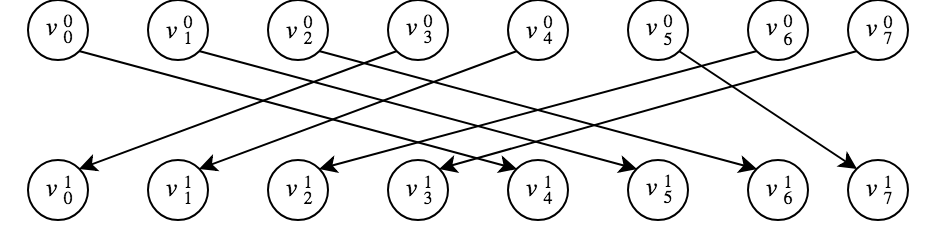
\includegraphics[width=\textwidth]{rp1.png}
	\centering	
	\caption{Graf utowrzony z Riffle-Permutation indukowanej przez $B=11100100$.}
	\label{2::im1}
\end{figure}

\begin{definition}[N-Single-Layer-Riffle-Graph] Niech $V = V^{0} \cup V^{1}$, gdzie $V^{i} = \{ v_{0}^{i},\dots,v_{N-1}^{i} \}$, niech $B$ będzie słowem binarnym długości $N$. Niech $\pi_{B}$ będzie Riffle-Permutaion indukowaną przez $B$.
	Graf N-Single-Layer-Riffle-Graph (dla parzystego N) zdefiniowany jest jako graf na wierzchołkach $V$ z następującymi krawędziami w zbiorze $E$:
	\begin{itemize}
		\item jedna krawędź: $v_{N-1}^{0} \rightarrow v_{0}^{1}$,
		
		\item $2(N - 1)$ krawędzi: $v_{i-1}^{j} \rightarrow v_{i}^{j}$, dla $i \in [N-1]$ oraz $j \in \{0, 1\}$,
		
		\item $N$ krawędzi: $v_{i}^{0} \rightarrow v_{\pi_{B}(i)}^{1}$, dla $i \in \{0,\dots,N -1\}$,
		
		\item $N$ krawędzi: $v_{i}^{0} \rightarrow v_{\pi_{\overline{B}}(i)}^{1}$, dla $i \in \{0,\dots,N -1\}$.
	\end{itemize}
\end{definition}

\begin{example}
	Kontynuując z danymi z przykładu \ref{2::p1},
		$\pi_{\overline{B}} = \bigl( \begin{smallmatrix}
	0 && 1 && 2 && 3 && 4 && 5 && 6 && 7 \\
	0 && 1 && 2 && 4 && 5 && 3 && 6 && 7
	\end{smallmatrix} \bigr) $.
	 8-Single-Layer-Riffle-Graph ukazany jest na rysunku \ref{2::im2}.
\end{example}

\begin{figure}[h]
	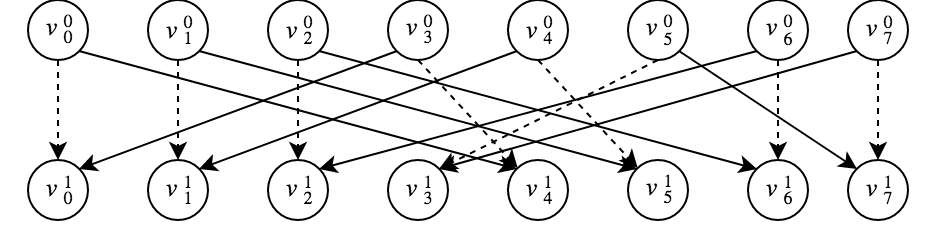
\includegraphics[width=\textwidth]{rp2.png}
	\centering
	\caption{8-Single-Layer-Riffle-Graph dla $B=11100100$ (krawędź $(v_{7}^{0}, v_{0}^{1})$ oraz krawędzie poziome zostały pominięte). Krawędzie dla permutacji $\pi_{B}$ oznaczone są linią ciągłą, a krawędzie dla permutacji $\pi_{\overline{B}}$ oznaczone są linią przerywaną.}
	\label{2::im2}
\end{figure}

\begin{definition}[N-Double-Riffle-Graph] \label{rs::ndrg} Niech $V$ oznacza zbiór wierzchołków, a $E$ zbiór krawędzi grafu $G =(V, E)$. Niech $B_{0},\dots,B_{g-1}$ będą wyrazami binarnymi o długości $N = 2^{g}$ każdy.
	N-Double-riffle-Graph jest otrzymywany poprzez ułożenie w stos $2g$ grafów, które spełniają warunki N-Single-Layer-Riffle-Graph. Otrzymany tak graf ma $(2g+1)2^{g}$ wierzchołków $ \{ v_{0}^{0}, \dots , v_{2^{g} - 1}^{0} \} \cup \dots \cup \{ v_{0}^{2g},\dots,v_{2^{g - 1}}^{2g} \} $,
	oraz następujące krawędzie:
	\begin{itemize}
		\item $(2g + 1)2^{g}$ krawędzi: $v_{i-1}^{j} \rightarrow v_{i}^{j}$ dla $i \in [2^{g}-1]$ i $j \in \{0,1,\dots,2^{g} \}$,
		
		\item $2g$ krawędzi: $v_{2^{g} - 1}^{j} \rightarrow v_{0}^{j+1}$ dla $j \in \{0,\dots,2g-1 \} $,
		
		\item $g2^{g}$ krawędzi: $v_{i}^{j-1} \rightarrow v_{\pi_{B_{j}}(i)}^{j}$, dla $i \in \{0,\dots,2^{g} -1\}$ i $j \in [g]$,
		
		\item $g2^{g}$ krawędzi: $v_{i}^{j-1} \rightarrow v_{\pi_{\overline{B}_{j}}(i)}^{j}$, dla $i \in \{0,\dots,2^{g} -1\}$ i $j \in [g]$,
	\end{itemize}
	oraz dla dolnych $g$ warstw, które są symetryczne względem warstwy $g$:
	\begin{itemize}
		\item $g2^{g}$ krawędzi: $v_{i}^{2g - j} \rightarrow v_{\pi_{B_{j}}^{-1}(i)}^{2g -j + 1}$, dla $i \in \{0,\dots,2^{g} -1\}$ i $j \in [g]$,

		\item $g2^{g}$ krawędzi: $v_{i}^{2g - j} \rightarrow v_{\pi_{\overline{B}_{j}}^{-1}(i)}^{2g - j + 1}$, dla $i \in \{0,\dots,2^{g} -1\}$ i $j \in [g]$,
	\end{itemize}

\end{definition}


\begin{definition}[(N,$\lambda$)-Double-Riffle-Graph] \label{rs::nldouble} Niech $G_{i}$, $i \in \{ 0,1,\dots,\lambda - 1\}$ będą N-Double-Riffle-Graph. Graf (N,$\lambda$)-Double-Riffle-Graph jest skonstruowany poprzez złączenie wyjść grafu $G_{i}$ do dopowiadających wejść grafu $G_{i+1}$, $i \in \{ 0, 1, \dots, \lambda - 2\}$.
\end{definition}

\subsection{Śledzienie trajektorii}
Graf jest generowany za pomocą permutacji pseudolosowej $\sigma$.
Ponieważ do generowania grafu potrzebne jest $g$ słów binarnych o długości $2^{g}$, a permutacje zawierają $2^{g}$ elementów, gdzie każdy ma maksymalnie $g$ bitów znaczących, trzeba przekształcić permutację tak, aby otrzymać pożądane dane.
Ta procedura nazwana jest śledzeniem trajektorii (ang. \textit{trace trajectories}).
Niech $B$ będzie macierzą binarną o rozmiarze $2^{g} \times g$, gdzie $j$-ta kolumna jest binarną postacią $\sigma(j) \in [2^{g}-1]$. Macierz $\mathfrak{B} = (\mathfrak{B}_{0},\dots,\mathfrak{B}_{g-1})$ oznaczać będzie transpozycję macierzy $B$, a więc macierz o potrzebnym do generacji grafu rozmiarze $g \times 2^{g}$.


\section{Tworzenie permutacji}

\subsection{Talia kart jako permutacja}
Początkową częścią funkcji $\mathbf{RiffleScrambler}$ jest generowanie permutacji na podstawie soli. Do utworzenia takiej permutacji używany jest algorytm $\mathbf{InverseRiffleShuffle}$, który imituje tasowanie kart do gry w odwrotnej kolejności.

Podczas tasowania talia kart dzielona jest na dwie części.
Podział odbywa się poprzez wybranie karty w środku talii, karty które są przed wybraną kartą tworzą pierwszą część, a pozostałe tworzą drugą część.
Następnie te dwie części są ze sobą łączone w jeden stos poprzez losowe umieszczanie karty z góry pierwszej lub drugiej części na stosie.
Można zauważyć, że kolejność kart wśród stosu z którego pochodzą nie zmienia się, lecz między kolejne karty z jednego stosu mogą wejść karty z drugiego.

W celu wygenerowania permutacji $N$ elementów, myślimy o tych elementach jako o kartach, a o permutacji, jako o pewnej ich kolejności.
Krok odwróconego sortowania wygląda następująco.

Dla każdej karty w talii losowany jest jeden bit, 0 lub 1. Wszystkie karty, dla których wylosowano 1 wyciągamy, zachowując ich kolejność i układamy na stos. Następnie umieszczamy ten stos na stosie kart, dla których wylosowano zera.

Dla każdego takiego kroku, dla każdej karty zapisywana jest informacja jaki bit został dla niej wylosowany. Zatem po $n$ krokach, każda karta ma przypisany ciąg binarny długości $n$.
Kończymy, kiedy talia kart jet dobrze posortowana, czyli kiedy każdej karcie przypisano unikalny ciąg binarny. Nowa kolejność elementów oznacza wygenerowaną permutację.

Można zauważyć, że liczba kroków tasowania $N$ kart na pewno nie będzie mniejsza od $\log{N}$, bo potrzebujemy $\log{N}$ bitów, aby każdej karcie przyporządkować inny ciąg binarny.

Algorytm $\mathbf{InverseRiffleShuffle}$ będzie mógł się zakończyć, kiedy każdy element będzie posiadał różny ciąg binarny. Średnio oznacza to $2 \log{N}$ kroków \cite{rs}.

\subsection{Algorytm generowania permutacji}
Razem z prezentacją RiffleScrambler zaproponowany został algorytm generowania permutacji \cite[Algorym 1]{rs}, który sprawdzał warunek końca w czasie $O(n^2)$ oraz potrzebował $O(n^2)$ komórek pamięci, gdzie $n$ oznacza wielkość permutacji.

Pseudokod [TODO...] przedstawia algorytm sprawdzający warunek końca w czasie $O(n)$ korzystając z $O(n log{n})$ komórek pamięci.

Algorytm opiera się na sortowaniu pozycyjnym radix sort \cite{radixsort}, gdzie jako pozycje sortowanych elementów podawane są losowane bity.
Permutowane elementy, trzymane są w tablicy, która jest sortowana po każdej iteracji dokładania kolejnego bitu. Dzięki temu sprawdzenie warunku końca odbywa się na posortowanej tablicy, którą wystarczy przejść sprawdzając czy każde dwa sąsiednie elementy są różne, co wykonywane jest w czasie liniowym.

\section{Algorytm}

Procedurę $\mathbf{RiffleScrambler}(pwd, s, g,\lambda)$ można z grubsza przedstawić następująco.

\begin{itemize}
	\item Dla podanej soli $s$ obliczana jest pseudolosowa permutacja $\sigma$ (używając algorytmu $\mathbf{InverseRiffleShuffle}$).
	
	\item Dla permutacji $\sigma$ tworzona jest macierz $\mathfrak{B} = \mathbf{TraceTrajectories}(B)$.
	
	\item Dla wyrazów binarnych $\mathfrak{B}_{0},\dots,\mathfrak{B}_{g-1}$ generowany jest graf $G$, który jest N-Double-Riffle-Graph. Przypomnijmy, $N = 2 ^ {g}$.
	
	\item Na grafie $G$ zainicjalizowanym wartością $pwd$, oblicze są wartości w ostatnim rzędzie ($v_{0}^{2g+1},\dots,v_{2^{g} - 1}^{2g + 1}$).
	
	\item Wartości z ostatniego rzędu przepisywane są do pierwszego, $v_{i}^{0} = v_{1}^{2g+1}$ dla $i \in \{ 0,\dots,2^{g}-1 \}$, a następnie znów oblicza się wartość ostatnich rzędów. Powtarzane jest $\lambda$ razy.
	
	\item Wartością końcową jest wartość w ostatnim wierzchołku, czyli w $v_{2^{g} - 1}^{2g}$.
\end{itemize}

\begin{example}[Generowanie (8,1)-Double-Riffle-Graph]
	Skoro $N = 8$, to $g = 3$, ponieważ $N = 2^g$. $\lambda = 1$.
	Niech otrzymaną permutacją $\sigma$ będzie $\bigl( \begin{smallmatrix}
	0 && 1 && 2 && 3 && 4 && 5 && 6 && 7 \\
	5 && 4 && 6 && 3 && 2 && 7 && 0 && 1
	\end{smallmatrix} \bigr) $.
	Zatem binarna postać permutacji $B = \bigl( \begin{smallmatrix}
		1 && 1 && 1 && 0 && 0 && 1 && 0 && 0 \\
		0 && 0 && 1 && 1 && 1 && 1 && 0 && 0 \\
		1 && 0 && 0 && 1 && 0 && 1 && 0 && 1
	\end{smallmatrix} \bigr) $.
	Przeprowadzając śledzenie trajektorii, czyli transponując $B$ otrzymujemy
	$\mathfrak{B} = (\mathfrak{B_0}, \mathfrak{B_1}, \mathfrak{B_2})$, $\mathfrak{B} =\bigl( \begin{smallmatrix}
	1 && 1 && 1 && 0 && 0 && 1 && 0 && 0 \\
	0 && 0 && 1 && 1 && 1 && 1 && 0 && 0 \\
	1 && 0 && 0 && 1 && 0 && 1 && 0 && 1
	\end{smallmatrix} \bigr)^{T} $.
	
	Teraz należy obliczyć permutacje $\pi_{\mathfrak{B_0}},\pi_{\mathfrak{B_1}},\pi_{\mathfrak{B_2}}$:
	
	$$ \pi_{\mathfrak{B_0}}=\bigl( \begin{smallmatrix}
	0 && 1 && 2 && 3 && 4 && 5 && 6 && 7 \\
	4 && 5 && 6 && 0 && 1 && 7 && 2 && 3
	\end{smallmatrix} \bigr), $$
		$$ \pi_{\mathfrak{B_1}}=\bigl( \begin{smallmatrix}
	0 && 1 && 2 && 3 && 4 && 5 && 6 && 7 \\
	0 && 1 && 4 && 5 && 6 && 7 && 2 && 3
	\end{smallmatrix} \bigr), $$
		$$ \pi_{\mathfrak{B_2}}=\bigl( \begin{smallmatrix}
	0 && 1 && 2 && 3 && 4 && 5 && 6 && 7 \\
	4 && 0 && 1 && 5 && 2 && 6 && 3 && 7
	\end{smallmatrix} \bigr). $$
	
	Wygenerowany graf z krawędziami zależnymi od permutacji ukazany jest na rysunku \ref{2::im3}.
	Dodając do niego krawędzie nie zależne od permutacji, otrzymujemy pełny graf (8,1)-Double-Riffle-Graph pokazany na rysunku \ref{2::im4}.
	
\end{example}


\begin{figure}
		\centering
		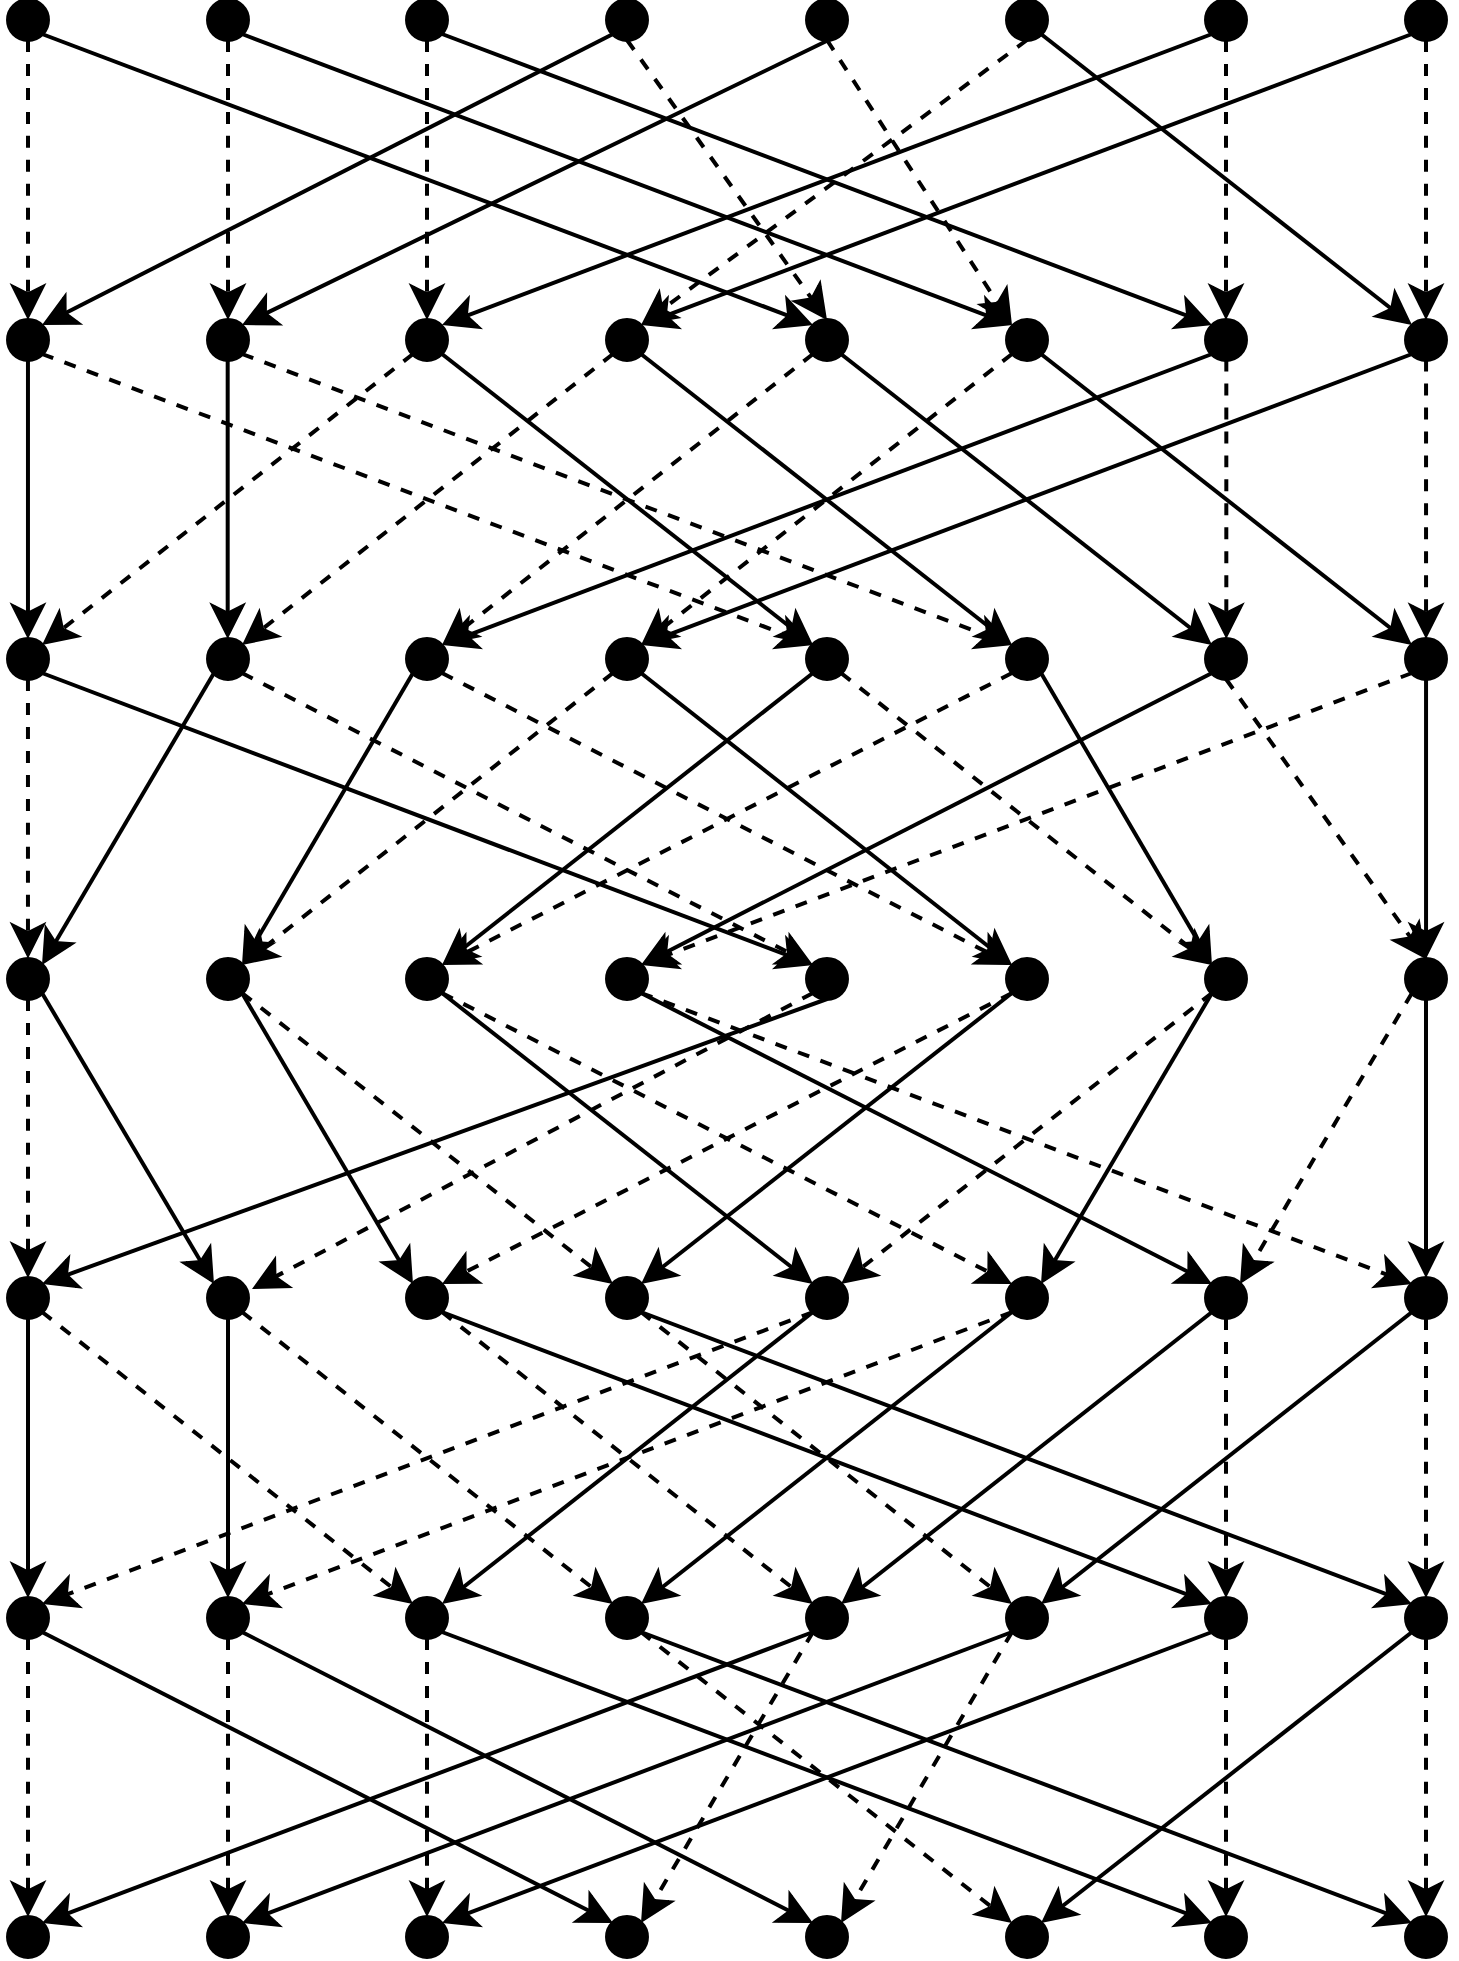
\includegraphics[width=0.7\textwidth]{all_rs1.png}

		\caption{(8,1)-Double-Riffle-Graph (krawędzie niezależne od permutacji, czyli przekątne oraz krawędzie poziome, zostały pominięte). Krawędzie dla permutacji oznaczone są linią ciągłą, a krawędzie dla permutacji negacji oznaczone są linią przerywaną.}
		\label{2::im3}
\end{figure}

\begin{figure}
	\centering
	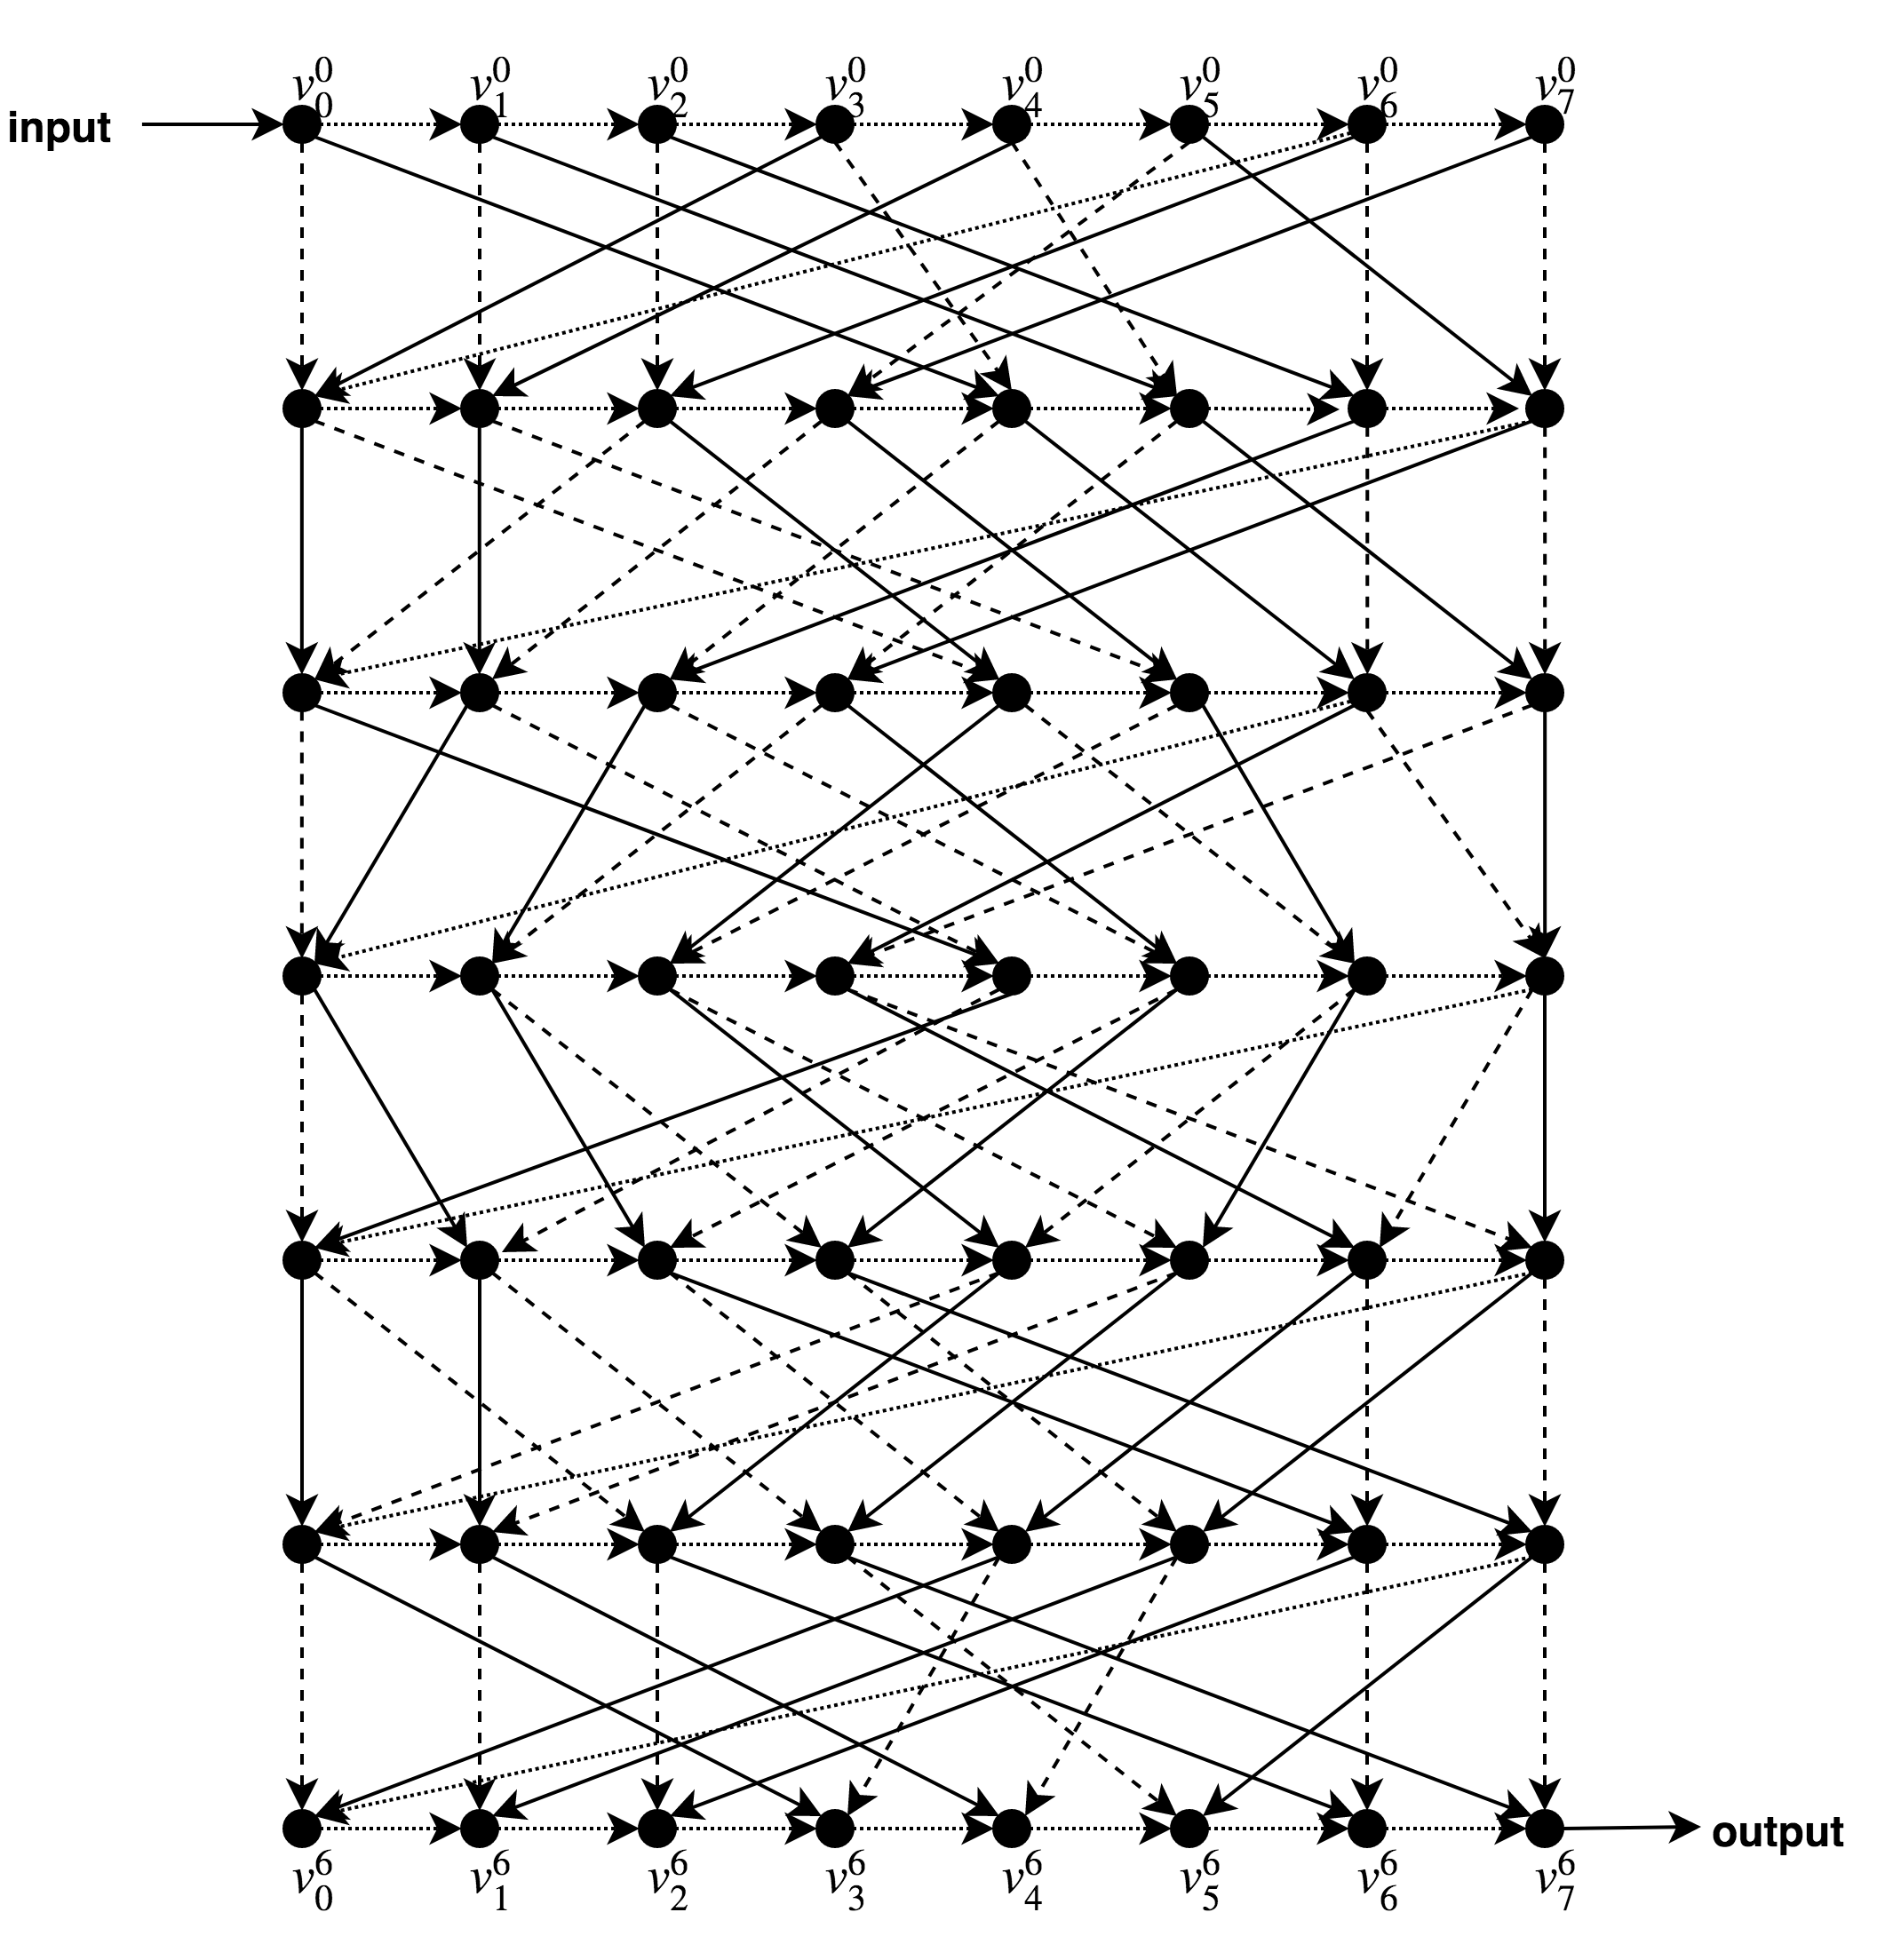
\includegraphics[width=\textwidth]{total_rs.png}
	
	\caption{(8,1)-Double-Riffle-Graph ze wszystkimi krawędziami oraz oznaczeniem wejścia i wyjścia. Krawędzie dla permutacji oznaczone są linią ciągłą, krawędzie dla permutacji negacji oznaczone są linią przerywaną, a krawędzie nie zależne od permutacji oznaczone są liniami kropkowanymi}
	\label{2::im4}
\end{figure}


\begin{algorithm}
	\caption{$\mathbf{RiffleShuffle}$}
	\SetAlgoLined
	\KwIn{N - wielkość premutacji do wygenerowania, getNextBit - generator bitów losowych}
	\KwOut{$\sigma$ - permtacja wielkości N}
	
	\tcc{$perm$ zawiera krotki będące początkowym indeksem oraz wyrazem binarnym.
	$perm[i] = (id, bin)$ dla $i\in \{0,\dots,N-1\}$}

	$perm = ((0, ````),(1,````),\dots,(N-1,````))$ \;
	
	\While{$\exists_{i \in \{0,\dots,N-2\}} perm[i][1] == perm[i+1][1]$}{
		$numberOfOnes = 0$ \;
		\For{$i = 0$ \KwTo $N - 1$}{
			$newBit = bitGenerator()$ \;
			$perm[i][1] = perm[i][1] + newBit$ \; 
			\If{$newBit == ``1``$}{
				$numberOfOnes = numberOfOnes + 1$ \;
			}
		}
		$lastIndexOfOnes = 0$ \;
		$lastIndexOfZeros = numOfOnes$ \;
		
		\For{$i = 0$ \KwTo $N - 1$}{
			\eIf{$lastBit(permutation[i][1]) == ``1``$}{
				$tmp[lastIndexOfOnes] = permutation[i]$ \;
				$lastIndexOfOnes = lastIndexOfOnes + 1$ \;	
			} {
				$tmp[lastIndexOfZeros] = permutation[i]$ \;
				$lastIndexOfZeros = lastIndexOfZeros + 1$ \;	
			}
		}
	
		$perm = tmp$ \;


	}
	$\sigma = (perm[0].id,perm[1].id,\dots,perm[N-1].id)$ \;
\end{algorithm}


\begin{algorithm}
	\caption{$\mathbf{GenGraph}$}
	\SetAlgoLined
	\KwIn{g - parametr wielkości grafu, $\sigma$ - permutacja wielkości $2^g$}
	\KwOut{G - graf na $2^g$ wierzchołkach z krawędziami wygenerowanymi na podstawie permutacji}
	
	$N = 2^g$ \;
	$V = \{ v_i^j: i \in \{0,\dots,N-1\}; j \in \{0,\dots, 2g \} \}$ \;
	$E = \{ v_i^j \rightarrow v_{i + 1}^{j} : i \in \{ 0, \dots, N - 2 \}; j \in  \{ 0, \dots, 2g \} \} $ \;
	$E = E \cup \{ v_{N-1}^{j} \rightarrow v_{0}^{j+1} : j \in \{ 0, \dots, 2g - 1 \} \}$ \;
	
	$\mathfrak{B} = (\mathfrak{B}_0,\dots,\mathfrak{B}_{g-1}) = \mathbf{TraceTrajectories}(\sigma)$ \;
	
	\For{$m = 0$ \KwTo $g - 2$}{
		$\mathfrak{B}_{2g + 1 - m} = \mathfrak{B}_{m}$ \; 
	}

	\tcc{Bity w słowach binarnych oznaczamy dodając indeks dolny. \
	$\mathfrak{B}_j = \mathfrak{B}_{j,0}\mathfrak{B}_{j,1}\dots \mathfrak{B}_{j,2^g-1}$
	}

	\For{$j = 0$ \KwTo $2g - 1$}{
		\For{$i = 0$ \KwTo $2^g - 1$}{
			
			$
			E = E \cup 
			\{ v_i^j \rightarrow v_{\pi_{\mathfrak{B}_{j,i}}}^{i+1} \}
			\cup \{ v_i^j \rightarrow v_{\pi_{\overline{\mathfrak{B}}_{j,i}}}^{i+1} \}$ \;
		}
	}
	$G = (V,E)$ \;
	
\end{algorithm}



\begin{algorithm}
	\caption{$\mathbf{RiffleScrambler}$}
	\SetAlgoLined
	\KwIn{s - sól, g - parametr wielkości grafu, pwd - hasło, $\lambda$ - ilość warstw w grafie, H - kryptograficzna funckja sktóru}
	\KwOut{pwd - hash podanego hasła}
	$\sigma = \mathbf{RiffleShuffle}(2^g, pseudoRandomBitGenerator(s,H))$ \;
	$G = (V,E) = \mathbf{GenGraph}(g, \sigma$) \;
	$v_0^0 = H(X)$ \;
	\For{$i = 1$ \KwTo $2^g-1$}{
		$v_i^0 = H(v_{i-1}^{0})$ \;
	}
	\For{$r = 1$ \KwTo $\lambda$}{
		\For{$j = 0$ \KwTo $2g$}{
			\For{$i = 0$ \KwTo $2^g-1$}{
				$v_i^{j+1} = 0$ \;
				\ForAll{$v \rightarrow v_i^{j+1} \in E$}{
					$v_i^{j+1} = H(v_i^{j+1}, v)$ \;
				}
			}	
		}
		\For{$i = 0$ \KwTo $2^g - 1$}{
			$v_i^0 = v_i^{2g+1}$ \;
		}
	}
	
	$hash = v_{2^g - 1}{2g}$ \;
\end{algorithm}

\section{Właściwości}

\begin{theorem} \label{rs::superk} \cite[Twierdzenie 5]{rs} Niech $\sigma$ będzie permutacją $N = 2^g$ elementów.
	Niech $G$ będzie N-Double-Riffle-Graph wygenerowanym dla $\mathfrak{B} = \mathbf{TraceTrajectories}(\sigma)$.
	Wtedy $G$ jest $N-Superkoncentratorem$.
\end{theorem}

\begin{theorem} \label{rs::rzed}
	$RSG_{\lambda}^{N}$ jest N rzędowym grafem.
\end{theorem}

\begin{proof}
	Z definicji $RSG_{\lambda}^{N}$ jest (N,$\lambda$)-Double-Riffle-Graph dla $N = 2^g$, a liczba wszystkich wierzchołków wynosi $n = (2g + 1)2^g$.
	Z definicji \ref{rs::ndrg} zawiera on ścieżkę przechodzącą przez $n$ wierzchołków $(v_{1},\dots,v_{n})$ oraz można rozłożyć graf na $N+1$ rzędów $V = V^{0} \cup \dots V^{2g}$, a krawędzie łączą jedynie wierzchołki w jednym rzędzie, lub łączą wierzchołki z rzędu $V^{i}$ z wierzchołkami z rzędu $V^{i+1}$ dla $i \in \{0,\dots,2g-1\}$. Zatem graf jest N rzędowy.
	
\end{proof}



\section{Ograniczenia złożoności RSG}

\begin{theorem} \label{rs::lower}
	Niech $ \lambda, n \in \mathbb{N}^{+}$ takie, że $n = \overline{n}(2 \lambda c + 1) $, gdzie $c \in \mathbb{N}$ i $ \overline{n} = 2^{c}$.
	Wtedy dla $ g = \lfloor \sqrt{ \overline{n}} \rfloor$
	$ RSG_{\lambda}^{ \overline{n}} \in \mathbb{D}_{1,g}^{\lambda, \overline{n}} $
	oraz
	$ \Pi_{cc}^{ \parallel }(RSG_{\lambda}^{\overline{n}}) = \Omega \left( \frac{n^{1.5}}{c \sqrt{c \lambda}} \right) $.
\end{theorem}

\begin{proof}
	Niech $G = RSG_{\lambda}^{ \overline{n}}$, niech $G_{1}, G_{2}, \dots , G_{ \lambda }$ będą
	podgrafami $G$ opisanymi w definicji \ref{rs::nldouble}.
	Pokażemy, że każdy $G_{i}$ jest (g, $\overline{n}$)-dispresed dla $g = \lfloor \sqrt{ \overline{n}} \rfloor $.
	
	Wybierzmy $i \in [ \lambda ]$ niech $L_{1}$ będzie ostatnimi $\overline{n}$ wierzchołkami w porządku topologicznym grafu $G_{i}$.
	Oznaczamy wierzchołki zbioru $L_{1}$ poprzez ${1} \times [ \overline{n} ]$, gdzie druga pozycja odpowiada kolejności wierzchołka w porządku topologicznym.
	Niech $ \overline{g} = \lfloor \overline{n} / g \rfloor$, dla każdego $j \in [ \overline{g}]$
	$L_{1, j} = \{ <1, jg + x> : x \in [0, g-1] \}$.
	Pokażemy, że wszystkie $L_{1, j}$ mają (g, g)-dependency.
	
	Niech $L_{0}$ będzie $\overline{n}$ pierwszymi wierzchołkami $G_{i}$, które oznaczamy ${0} \times [\overline{n}]$ (ponownie druga pozycja odpowiada porządkowi topograficznemu).
	Zauważmy, że dla $n \textgreater 1$ i $g = \lfloor \sqrt{ \overline{n}} \rfloor$ prawdą jest, że $g(g - 2c + 1) \leq n$.
	Zatem zbiór $S = \{ <0, i(g - 2c + 1_)>: i \in [g] \}$ jest całkowicie zawarty w $L_{0}$.
	
	Z twierdzenia \ref{rs::superk} mówiącym, że $RSG$ jest N-Superkoncentratorem wynika, że skoro zbiory $S$ oraz $L_{1,j}$ mają po $g$ wierzchołków, to istnieje $g$ wierzchołkowo-rozłącznych ścieżek o długości $2c$ między wierzchołkami tych zbiorów. Zatem $L_{1,j}$ ma (g, 2c)-dependency.
	
	Rozszerzmy to do (g,g)-dependency.
	Niech ścieżka $p$ zaczynająca się w wierzchołku $<0, v> \in S$ będzie ścieżką w (g, 2c)-dependency $L_{1,j}$. Zauważmy, że istnieje ścieżka przechodząca przez wszystkie wierzchołki $L_{0}$ oraz, że wierzchołki zbiory $S$ są oddzielone między sobą o $g - 2c$ wierzchołków.
	Możemy dodać na początek ścieżki $p$ ścieżkę $( <0, v - (g - 2c - 1)>, <0, v - (g - 2c -2)>, \dots, <0, v>)$.
	Otrzymujemy w ten sposób ścieżkę $p_{+}$ o długości $2c + g - 2c = g$.
	Ponieważ każda para ścieżek $p \neq q$ w (g, 2c)-dependency $L_{1,j}$ jest wierzchołkowo-rozłączna,
	to w szczególności zaczynać się muszą w różnych wierzchołkach $<0, v_{p}> \neq <0, v_{q}>$.
	Ponieważ wierzchołki w $S$ są od siebie oddalone o $g - 2c$ wierzchołków, zatem ścieżki $p^{+}$ i $q_{+}$ nadal pozostają rozłączne.
	Rozszerzając w ten sposób wszystkie ścieżki z (g, 2c)-dependency otrzymujemy ścieżki wierzchołkowo-rozłączne długości $g$. Z tego wynika, że $L_{1,j}$ ma (g, g)-dependency, co dowodzi, że $ RSG_{\lambda}^{ \overline{n}} \in \mathbb{D}_{1,g}^{\lambda, \overline{n}} $.
	Pozostaje obliczyć górne ograniczenie używając twierdzenia \ref{1::disp}.
	
	$$ \Pi_{cc}^{ \parallel }(RSG_{\lambda}^{\overline{n}}) = \lambda g \left( \frac{ \overline{n}}{2} - g \right) \geq \lambda \lfloor \sqrt{ \overline{n}} \rfloor \left( \frac{ \overline{n}}{2} - \lfloor \sqrt{ \overline{n}} \rfloor \right) = \lambda \sqrt{ \overline{n}} \left( \frac{ \overline{n}}{2} - \sqrt{ \overline{n}} \right) - O(\overline{n}) =  \Omega \left( \lambda \overline{n} \right) = \Omega \left( \frac{n^{1.5}}{c \sqrt{c \lambda}} \right) $$
	
\end{proof}



\begin{theorem} \label{rs::upper}
	Niech $\lambda, g \in \mathbb{N}^{+}$, $N = 2^{g}$, $n = N(2 \lambda g + 1)$, wtedy
	$$ \Pi_{cc}^{ \parallel }(RSG_{\lambda}^{\overline{n}}) = O \left( n^{1.667} \right) $$
\end{theorem}

\begin{proof}
	Kożystając, z twierdzenia \ref{rs::rzed}, $RSG_{\lambda}^{N}$ jest $N$ rzędowym grafem.
	Z lematu 2.2 wynika więc, że $RSG_{\lambda}^{N}$  jest ($n / t$, $N + t - N - 1$)-reducible dla dowolnego $t \geq 1$.
	Z lematu \ref{1::rze} wynika, że $\Pi_{cc}^{ \parallel }(RSG_{\lambda}^{\overline{n}}) = O \left( n \left( \sqrt{( N t + t - N - 1)n \delta } + \frac{n}{t} \right) \right)$.
	Aby dostać najdokładniejsze (najmniejsze) ograniczenie górne trzeba zminimalizować
	$n \left( \sqrt{( N t + t - N - 1)n \delta } + \frac{n}{t} \right)$.
	Zanim jednak przejdziemy do minimalizowania, uprośćmy nieco to wyrażenie
	$$ n \left( \sqrt{( N t + t - N - 1)n \delta } + \frac{n}{t} \right) \leq n \left( \sqrt{ 2N t n \delta } + \frac{n}{t} \right) .$$
	Teraz możemy znaleźć minimum względem naszego parametru $t$.
	$$ \frac{\partial}{\partial t} n \left( \sqrt{( 2N t)n \delta } + \frac{n}{t} \right) = \frac{ \sqrt{ 2 \delta N n^{3} }}{2t} - \frac{n^{2}}{t^{2}}$$
	Minimum znajduje się w punkcje, gdzie pochodna ma wartość zero.
	$$ \frac{ \sqrt{ 2 \delta N n^{3} }}{2t} - \frac{n^{2}}{t^{2}} = 0$$
	$$ t = \frac{2n^{2}}{ \sqrt{ 2 \delta N n^{3} }} = O \left( n^{\frac{1}{3}} \right) $$
	Zatem podstawiając $t$ minimalizujące ograniczenie górne do wzoru z twierdzenia \ref{1::redu} otrzymujemy
	$$ \Pi_{cc}^{ \parallel }(RSG_{\lambda}^{\overline{n}}) = O \left( n \left( \sqrt{( N n^{\frac{1}{3}} + n^{\frac{1}{3}} - N - 1)n \delta } + \frac{n}{n^{\frac{1}{3}}} \right) \right) = O \left( n^{1.667} \right). $$
\end{proof}

\section{Porówanie}

MHF można porównywać za pomocą złożoności całkowitej, która mówi o koszcie równoległego obliczania funkcji.
Im ta złożoność jest wyższa, tym bardziej czas obliczeń jest zdominowany przez koszt dostępu do pamięci, a więc funkcja jest bezpieczniejsza. Porównanie przedstawione jest w tabeli \ref{2::tab2}.

\begin{table}[H]
	\centering
	\begin{tabular}{|c | c | c |} 
		\hline
		Algorytm & Ograniczenie dolne & Ograniczenie górne\\
		\hline
		Argon2i-B & $\Omega(n^{1.667})$ & $O(n^{1.8})$ \\
		\hline
		Catena Butterfly & $\Omega(n^{1.5})$ & $O(n^{1.625})$ \\
		\hline
		RiffleScrambler & $\Omega(n^{1.5})$ & $O(n^{1.667})$ \\
		\hline
	\end{tabular}
	\caption{\cite[Tablica 1]{depth} Porównianie złożoności całkowitej dla Argon2i, Catena (dla grafu Butterfly) oraz RiddleScrambler (Twierdzenia  \ref{rs::lower}, \ref{rs::upper}).}
	\label{2::tab2}
\end{table}


 Ważnym aspektem jest również czas obliczeń, czyli w ilu krokach można obliczyć daną funkcję. Ponieważ koszt obliczania funkcji ma pochodzić głównie z kosztu dostępu do pamięci, to czas obliczeń może zostać zminimalizowany. Jednocześnie przy próbie obliczenia funkcji z mniejszą, niż wymaganą ilością pamięci, czas obliczeń powinien rosnąć jak najszybciej, tak aby wymuszać użycie założonej ilości pamięci.
 Tablica \ref{2::tab} zawiera porównanie właściwości czasu obliczeń (etykietowania) T w zależności od dostępnej pamięci S (ilości etykiet).
 

\begin{table}[H]
	\centering
\begin{tabular}{|c | c | c | c | c | c|} 
	\hline
	 & $BHF_7$ & $BHG_3$ & Argon2i & Catena BFG & RiffleScrambler \\
	 	\hline
	Czas obliczeń T dla S = N & $8\lambda N$ & $4 \lambda N $ & $2 \lambda N$  & $4 \lambda N$ & $3 \lambda N$ \\
	 	\hline
	Czas obliczeń T dla $S \leq \frac{N}{64}$ & $T \geq \frac{2^{\lambda}-1}{32S} N^{2}$ & $T \geq \frac{\lambda N^2}{32S}$ & $T \geq \frac{ N^2}{1536S}$  & $T \geq \left( \frac{\lambda N^2}{64S} \right)^{\lambda}$ & $T \geq \left( \frac{\lambda N^2}{64S} \right)^{\lambda}$ \\
	Czas obliczeń T dla $\frac{N}{64} \leq S \leq \frac{N}{20}$ & nieznany & \\
	 	\hline
	Graf zależny od soli & tak & tak & tak  & nie & tak \\
	\hline

\end{tabular}
	\caption{ \cite[Tablica 4]{rs} Porównianie bezpieczeństwa i wydajności dla Balloon Hashing($BHF_7$ dla grafu o stopniu wejściowym 7,  $BHF_3$ dla grafu o stopniu wejściowym 3), Argon2i, Catena (dla grafu Butterfly) oraz RiffleScrambler.}
		\label{2::tab}
\end{table}





